Modern computing devices are becoming ever smaller, and to remain functional they must be engineered to combat the encroaching quantum effects at these scales, with increasing difficulty. Intel's current process incorporates a 14nm FET channel, as such the design of these FETs has been greatly changed to eliminate quantum effects. \cite{intel_process} In the near future, Intel will continue moving to a 10nm process which is presenting with further challenges. \cite{intel_future}

The trend in transistor miniaturisation has been dubbed "Moore's Law", following a prediction made by Gordon Moore, co-founder of Intel, in 1965. \cite{moores_law}

\begin{quotation}
	"The complexity for minimum component costs has increased at a rate of roughly a factor of
	 two per year ... Certainly over the short term this rate
	can be expected to continue, if not to increase." 
\end{quotation}
 Despite the remarkable accuracy of this prediction, many believe \cite{end_of_Moore_1, end_of_Moore_2} the inevitable breakdown of this rule will take place as the physical limitations of creating such devices exponentially increases the start-up cost of manufacturing, as well as the cost of research and development.

However, this brick-wall has sparked research into alternative forms of computation. One such example, is a general purpose quantum computer. A quantum computer is unlike any classical computer, in the sense that its principles of operation are entirely based on quantum mechanics, as opposed to the classical electronics which modern computers are designed from. The difference between these paradigms cannot be understated, and one is not simply a replacement for the other. Despite the lack of a working quantum computer at this point in time, many researchers have spent time designing certain algorithms and processes that would run on such a machine, and analysing the benefits of the architecture compared to the classical computer. One such example is Grover's algorithm \cite{grovers_algorithm}, which is a method to sort databases which has a worst-case execution time of $\mathcal{O}(\sqrt{n})$, a remarkable improvement over the theoretical limit of any classical comparison based algorithm, $\mathcal{O}(n \log{n})$.


\todo[inline]{Introduce the work I'm doing, in particular. Describe structure of document}

\begin{figure}[htbp!]
	\centering
	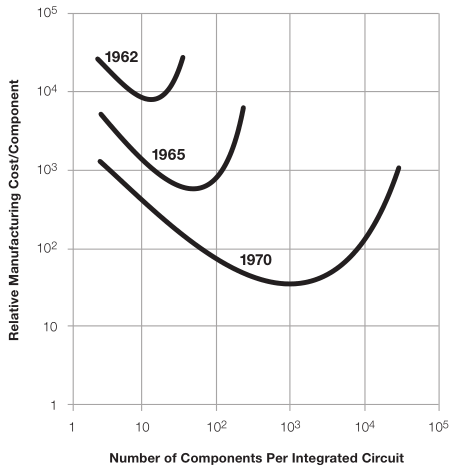
\includegraphics[width=0.8\textwidth]{moores_law}
	\caption{Gordon Moore's Prediction on Component Cost - Moore's Law}
	\label{fig::moores_law}
\end{figure}
